\documentclass[conference,compsoc]{IEEEtran}
\usepackage{comment}
\usepackage{subfigure}
\usepackage{enumitem}
\usepackage[ruled,vlined,linesnumbered]{algorithm2e}
\usepackage{algorithmic}

\usepackage{bm}%used for bm
\usepackage{graphics}
\usepackage{graphicx}
\usepackage{amsmath} %used for maths symbols
\usepackage{amssymb}%used for empty set symbol
\usepackage{url}
\usepackage{xcolor}% or package color

%used for quotes
\usepackage{epigraph}
\setlength\epigraphwidth{\columnwidth}
\setlength\epigraphrule{0pt}

\usepackage{array}
\newcolumntype{L}[1]{>{\raggedright\let\newline\\\arraybackslash\hspace{0pt}}m{#1}}
\newcolumntype{C}[1]{>{\centering\let\newline\\\arraybackslash\hspace{0pt}}m{#1}}
\newcolumntype{R}[1]{>{\raggedleft\let\newline\\\arraybackslash\hspace{0pt}}m{#1}}

\begin{document}


\title{Normal States Training for High Accuracy Event Detection}

\maketitle
\begin{abstract}
In the news value theory, the \textit{news unexpectedness} expects the journalists to report the events that are different from the routine things, a.k.a., the normal states. 
For human being, normal states are knowledge learned from news streams and the external environment, and can describe what happened and help to identify what is happening.
In this paper, we propose \textsc{NSDetector}, a high accuracy event detection method that trains normal states better by using knowledge base, which can be treated as the accumulation of happened things. 
%TODO
In \textsc{NSDetector}, 1) balanced for effectiveness and efficiency, normal states are trained as topical words and their chi-squared scores, and initialized by knowledge base; 2) topical word frequencies on targeted corpus within the time window are learned by NS-Prior-LDA, using the normal states as prior; 3) events are detected by monitoring the change of topical word frequencies; 4) normal states are further maintained by detected events incrementally.
Experiments on the benchmark \textit{Edinburgh twitter corpus (30 million tweets)} validate the effectiveness of our proposed \textsc{NSDetector}.
%\textsc{NSDetector} imitates this process automatically in the event detection task, and further verify that the key to improve the accuracy of event detection lies in training the normal states well. 
\end{abstract}

%\textsc{NSDetector} imitates this process automatically in the event detection task, and further verify that the key to improve the accuracy of event detection lies in training the normal states well. 

\section{Introduction}
%\textit{``To study the abnormal is the best way of understanding the normal."}---William James
%\textit{``The unpredictable or the rare is more newsworthy than the routine."}---Allan Bell

%The event detection task always tries to find out the newsworthy messages from cyberspace. 
With the increasing of cyberspace data, there is a growing need for detecting events accurately. Detecting events can mainly benefit the following three folds: (1) understanding what happened in the corpus without checking every single document manually, and generating the timeline to get a bird's eye view of the corpus\cite{ge2015bring}; (2) being aware what is happening currently, which helps to deal with emergencies\cite{hughes2009twitter}\cite{sakaki2010earthquake}; (3) adding detected events and their types as extra structured data information to organize the unstructured text corpus\cite{ritter2012open}.  

Considering the importance of event detection on the cyberspace data, researchers have have made many efforts, including checking the and the . Therefore, the existing methods are ... and 

In our study, we find out that the key to improve the accuracy of event detection lies in training the normal states of the focused media/site/domain. Based on training normal states accurately, event detection task can be treated as finding terms, articles, or topics which are different from the normal states. 

Our intuition is inspired from the news value theory\cite{galtung1965structure}\cite{caple2013delving}, which emphasizes the \textit{news unexpectedness} -- "the unpredictable or the rare is more newsworthy than the routine"\cite{bell1991language}, and "routine events are difficult to assimilate to the news, which favours the novel, the atypical and the unusual"\cite{montgomery2007discourse}.
Following this guideline, if the journalist knew the normal states, aka, the "routine things" of everyday better, he/she would tend to choose more unexpected news to report. 
We suppose that the ideal event detection system performs like a journalist who can find news from cyberspace with the knowledge of the normal states. 

\begin{figure}
    \label{fig:modelDesc}
    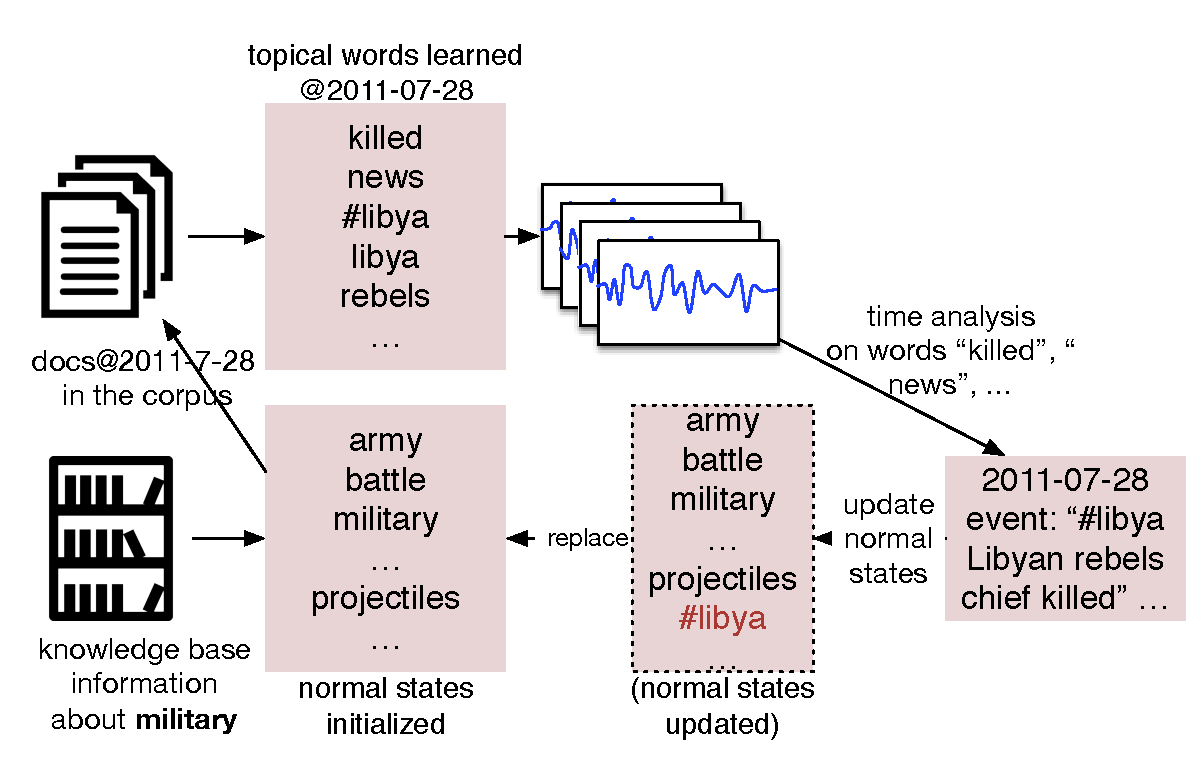
\includegraphics[width=1.0\columnwidth]{img/NSDetectorExample.pdf}
    \caption{\textsc{NSDetector}'s process flow, taking \textbf{military} related events in cyberspace as an example. \textsc{NSDetector} initializes the normal states about military from knowledge base, learns the topical words further within the time windows on the target corpus, detects events, and updates the normal states incrementally by the detected events.}
\end{figure}

For example, in ideal conditions an event detection system for anti-terrorism has the knowledge about the normal state such as “the words ISIS and Syria are both high-frequent, while the word Russia is not so frequent as them”. 
With the knowledge of normal state, the system for anti-terrorism can detect the event of “Russia's anti-ISIS op in Syria” as Russia appeared more frequent than the normal state and appeared with ISIS and Syria. 
After detection, the ideal event detection system also updates the normal state by considering the new coming data.



\section{Related Works}
\subsection{Event Detection}

To train the normal states, the methods of existing systems can be grouped into unsupervised methods and supervised methods based on whether they .

In the first category, the methods treat the normal states as clustered articles\cite{Petrovic:2010uj}\cite{Wurzer:2015wq}, word frequencies\cite{Mathioudakis:2010fc}\cite{Weng:2011wz}, or topics\cite{Diao:2012wj}\cite{Yan:2015wm}. 
Taking the clustering of articles\cite{Petrovic:2010uj}\cite{Wurzer:2015wq} as an example, they model the occurred events as clusters, and link the incoming article with an existing event cluster or assign it as the new detected event.
The decision is based on whether the dissimilarity between the incoming article and existing event clusters is over the user-specified threshold. 

And in the second category, the methods learn the normal states by given the knowledge of \textit{event trigger}\cite{Li2013JointEE}\cite{Nguyen2015EventDA} (usually a single verb or entity mentions). The normal states are trained by the labeled data appeared in a fixed time window.

Both categories of methods have achieved good performance on formal texts, but are hampered by the diverse and rapid changing nature of cyberspace data (e.g., twitter\cite{Asur:2011tc} and reddit\cite{singer2014evolution}).
In the journalist metaphor of news value theory, they have the limited knowledge of normal states (aka "routine things") due to the limited history information used. 
More specifically, 

The second category, train the triggers\cite{Li2013JointEE}\cite{Nguyen2015EventDA}(\textit{But it has some problems here, these methods are used in event extraction, so what's the relationship between event extraction and event detection? and the fired example in \cite{Li2013JointEE}?}). 


Although \cite{Wurzer:2015wq} points out that UMass\cite{Allan:2000wu} and its variants\cite{Petrovic:2010uj}\cite{petrovic2012using}\cite{Wurzer:2015wq} are the state-of-art systems on the Event Detection task for the newswire data, these systems still suffers from the lack of accuracy to applied on more general cyberspace data, such as tweets, emails, and reddit posts. 
The underlying reason is that the normalized Topic Weighted Minimum Cost metric (\(C_{min}\)) used in the Event Detection keep balance between miss and false alarm, which cannot work well on the .
Usually these traditional systems set the ratio of cost between miss alarm and false alarm to 10, preferring recall to precision on detecting events.

Study of event detection on text stream can be divided into three ways: word frequency based, text similarity based and topic model based.

Several word frequency methods have been developed for event detection such as Discrete Fourier Transform\cite{he2007analyzingDFT}, wavelet analysis \cite{weng2011eventWavelet}.
They treat the word's document frequency along timeline as time series and do the analysis in frequency domain. 
DFT method suffers the problem that it can not locate the time point for bursty, while wavelet analysis based method's complexity is very high, which limits its scalability. 

 Text similarity based online event detection methods\cite{petrovic2010streaming}\cite{mccreadie2013scalable}  suffer from the lexical variation which means different words describe the same events.
 Similarity based method can successfully detect the tweet which is retweeted by many times, but fails to find out the event which is described from many different perspectives.
 As a result, many events are duplicately detected due to their popularities, which may bury other events and overwhelm users with duplicated unwanted content.


In contrast, topic model can handle the lexical variation problem with word co-occurrence\cite{blei2003latent}.
%After \cite{blei2006dynamic} and \cite{wang2006topics} introducing time factor into topic model, a number of temporal model has been developed to different tasks.
As many events are highly related to topics, a number of methods based on topic model have been proposed for event detection, including online detection and offline detection.
Lau\cite{lau2012line} introduces an online topic model to track emerging events in microblogs.
It can deal with a massive of tweets, but it doesn't filter out the tweets related to user interests.
Diao\cite{timeUserLDA2012finding}\cite{diao2013unified} show that event detection can benefit from filtering out user interest related tweets. 
And Yan\cite{Yan:2015wm} models the bursty topic by incorporating burstiness of biterms as prior knowledge.
But they are different from ours.
As these models need the whole dataset as the input, they are offline detections, which is not scalability for large dynamic dataset such as microblogs.
\subsection{Knowledge Base}


%Twitter Trending Topic Classification
%We use PageRank-HITS\cite{Yan:2015wq} algorithm to update score of categories in wikipedia.

%3*4 figures, 0-11 is reorganized in the following order: 0, 1, 4, 5, 8, 9;
%2, 3, 6, 7, 10, 11;
\begin{figure*}[ht]
        \centering
        \label{fig:subfig} %% label for entire figure
        \subfigure[\((0.25,0.25,0.25)\)]{
                \label{fig:subfig:a} %% label for first subfigure a
                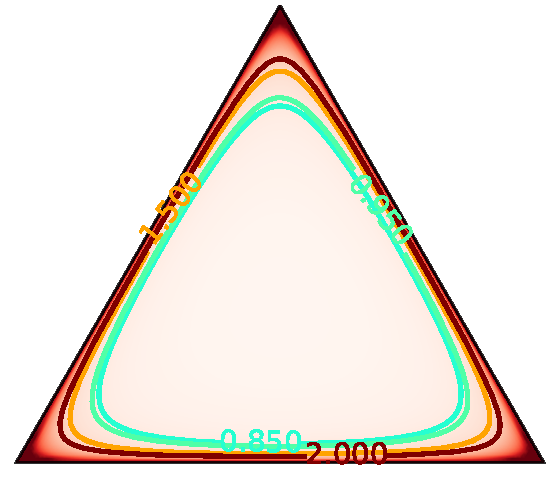
\includegraphics[height=2.14cm]{img/croppedDirichletGraph0.pdf}
        }
        \subfigure[\((0.5,0.5,0.5)\)]{
                \label{fig:subfig:b} %% label for second subfigure b
                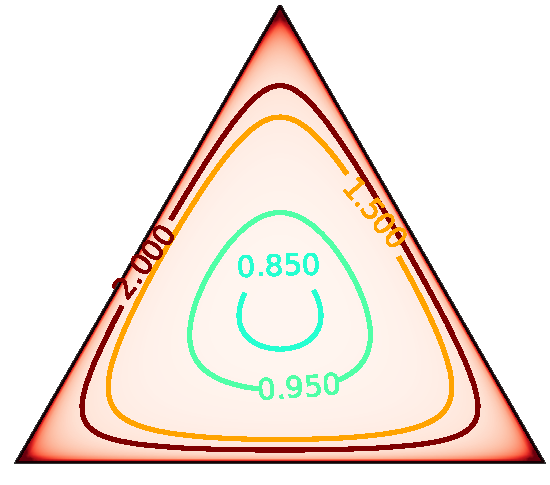
\includegraphics[height=2.14cm]{img/croppedDirichletGraph1.pdf}
        } 
        \subfigure[\((0.25,0.25,0.75)\)]{
                \label{fig:subfig:c} %% label for third subfigure c
                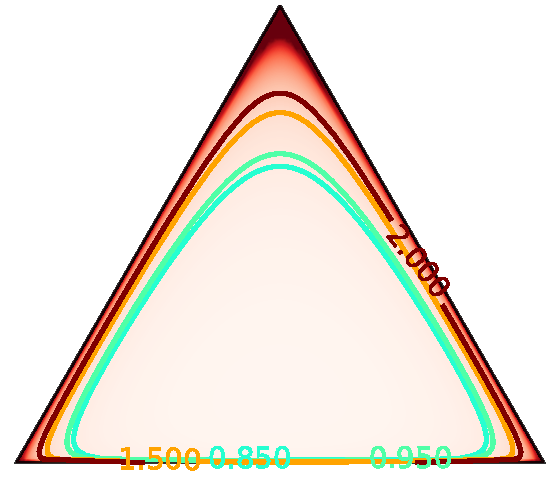
\includegraphics[height=2.14cm]{img/croppedDirichletGraph4.pdf}
        }
        \subfigure[\((0.5,0.5,1.5)\)]{
                \label{fig:subfig:a} %% label for first subfigure d
                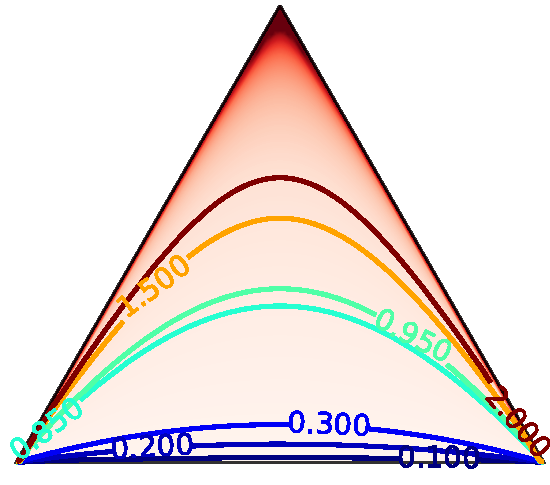
\includegraphics[height=2.14cm]{img/croppedDirichletGraph5.pdf}
        }
        \subfigure[\((0.25,0.75,0.75)\)]{
                \label{fig:subfig:d} %% label for third subfigure e
                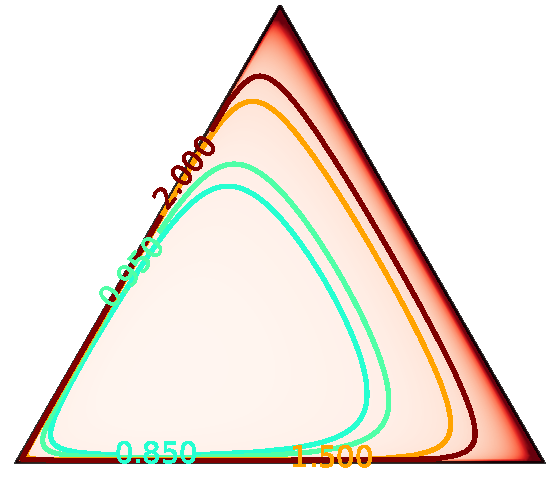
\includegraphics[height=2.14cm]{img/croppedDirichletGraph8.pdf}
        }
        \subfigure[\((0.5,1.5,1.5)\)]{
                \label{fig:subfig:d} %% label for third subfigure f
                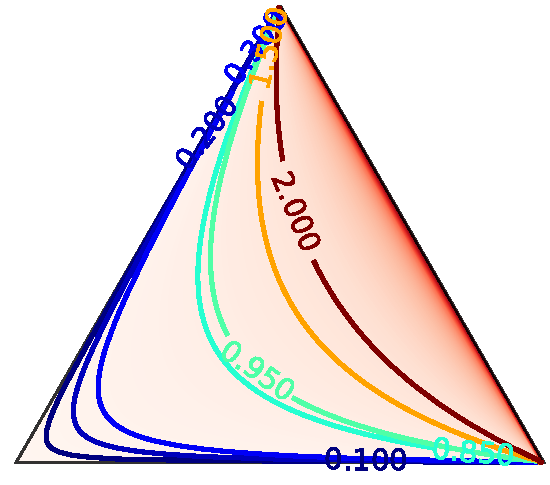
\includegraphics[height=2.14cm]{img/croppedDirichletGraph9.pdf}
        }\hspace{1in}
        \subfigure[\((1.5,1.5,1.5)\)]{
                \label{fig:subfig:d} %% label for third subfigure g
                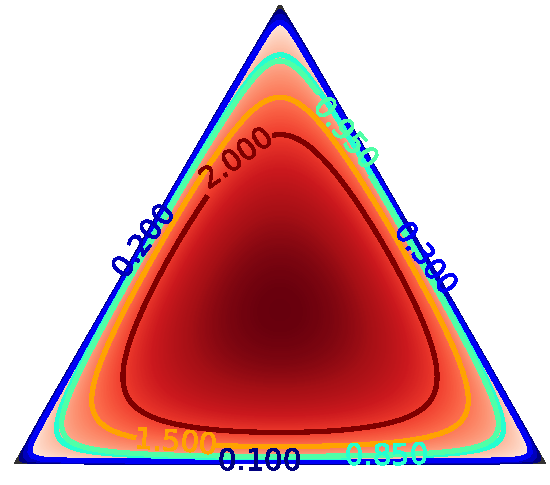
\includegraphics[height=2.14cm]{img/croppedDirichletGraph2.pdf}
        }
        \subfigure[\((2.5,2.5,2.5)\)]{
                \label{fig:subfig:a} %% label for first subfigure h
                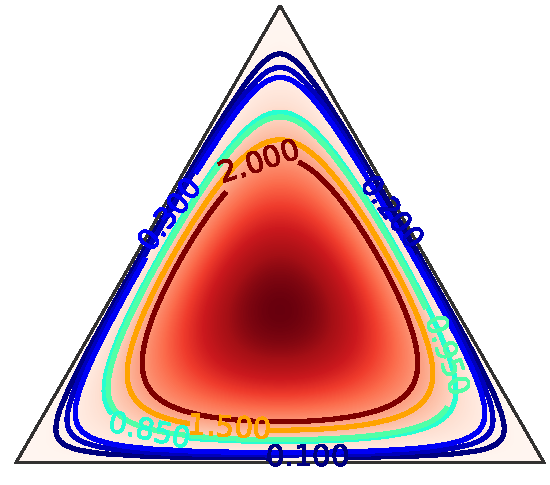
\includegraphics[height=2.14cm]{img/croppedDirichletGraph3.pdf}
        }
        \subfigure[\((1.5,1.5,2.5)\)]{
                \label{fig:subfig:d} %% label for third subfigure i
                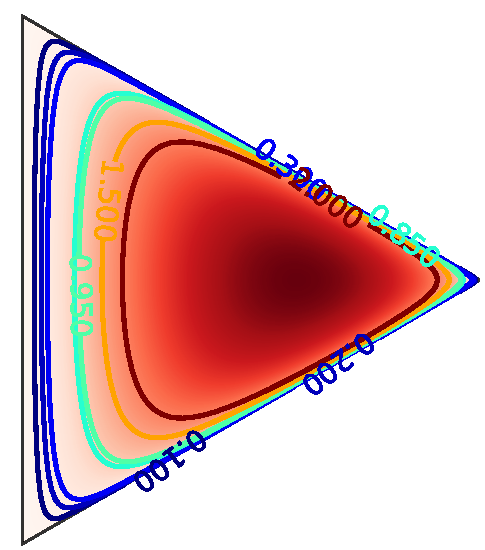
\includegraphics[height=2.14cm]{img/croppedDirichletGraph6.pdf}
        }
        \subfigure[\((2.5,2.5,3.5)\)]{
                \label{fig:subfig:d} %% label for third subfigure j
                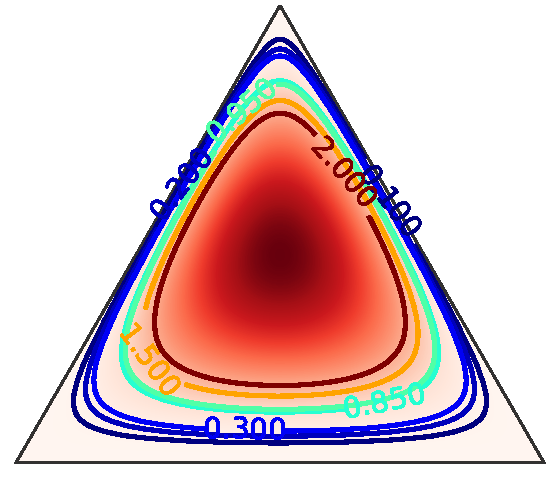
\includegraphics[height=2.14cm]{img/croppedDirichletGraph7.pdf}
        }
        \subfigure[\((1.5,2.5,2.5)\)]{
                \label{fig:subfig:d} %% label for third subfigure k
                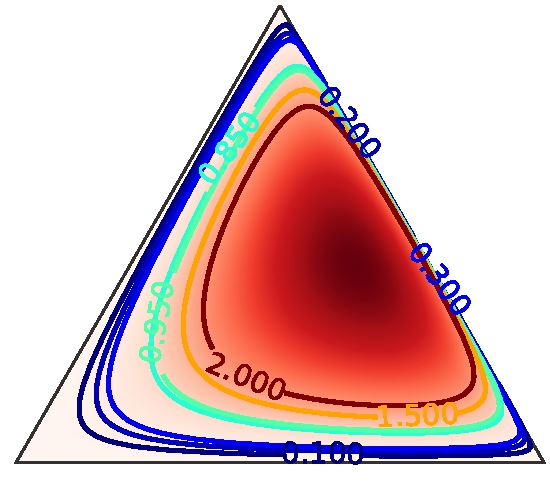
\includegraphics[height=2.14cm]{img/croppedDirichletGraph10.pdf}
        }
        \subfigure[\((2.5,3.5,3.5)\)]{
                \label{fig:subfig:a} %% label for first subfigure l
                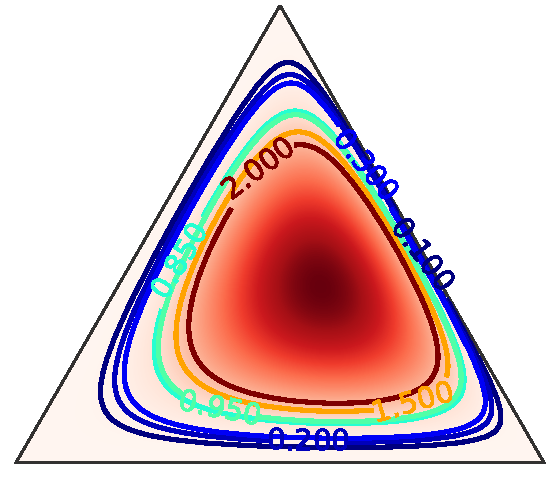
\includegraphics[height=2.14cm]{img/croppedDirichletGraph11.pdf}
        }\hspace{1in}
        \caption{Illustration of Dirichlet distribution's probabilistic density on the 3-dimensional simplex when given different priors. (a,b,g,h) the left four subfigures illustrate the probabilistic density when given the symetric priors for Dirichlet distribution; (c,d,i,j) the central subfigures illustrate the probablistic density given ; (e,f,k,l) }
\end{figure*}



\section{Proposed Method}
\begin{algorithm}
\caption{Overview of \textsc{NSDetector}}
\label{alg:overviewNSDetector}
\KwIn{Knowledge Base's structure \(G^{(0)}\), \(G^{(1)}\), and content \(G^{(2)}\), }
\KwOut{Events}
\(n_{k,t}\)=number of connected component in \(\mathcal{G}_{k,t}\)\\
\For{\(n \in \{ n_{k,t}, \cdots, |\mathcal{G}_{k,t}|\}\) }{
    \(\mathcal{C}_{k,t}=SpectralClustering(\mathcal{G}_{k,t},n)\)\\
    \If{\(min_{i\in \{1,\cdots,n\}} Density(\mathcal{C}_{k,t,i},\mathcal{G}_{k,t})>\tau\)}{
        return \(\mathcal{C}_{k,t}\)
    }
}
\end{algorithm}


\subsection{Initialization of Normal States}
In this part, we discuss in detail how to initialize the normal states from the given knowledge base. 
\begin{algorithm}
\caption{Normal States' Initialization from Knowledge Base}
\label{alg:normalStatesInit}

\KwIn{Taxonomy's Directed Acyclic Graph \(G^{(0)}\), Category-Page Bipartite Graph \(G^{(1)}\), Page-Content Bipartite Graph \(G^{(2)}\), topic related category node \(c\)}
\KwOut{Normal states \(\bm{f}_c\) on topic \(c\)}
\(Pages(c)\leftarrow \varnothing\)\\
\(SuccessorNodes(c) \leftarrow \) Breadth-first-search(\(G^{(0)},c\))\\
\For{\(node \in SuccessorNodes(c)\)}{
    \(Pages(c) \leftarrow Pages(c) \cup G^{(1)}.neighbours(node)\)\\
}
\(WordFrequencyTable(c) \leftarrow \) do word count on the text contents of \(Pages(c)\) \\
\(WordFrequencyTable(All) \leftarrow \) do word count on the text contents of all pages in \(G^{(2)}\).\\
\For{word \(w\) in WordFrequencyTable(All).keys()}{
    \(\tau_{c,w} \leftarrow \) \(w\)'s chi-square score on \(WordFrequencyTable(c)\) and \(WordFrequencyTable(All)\).
}
\Return{\(\bm{f}_c\)}
\end{algorithm}

\cite{faralli2015large} propose the Twixonomy Graph. 

%TODO

\begin{figure}
    \centering
    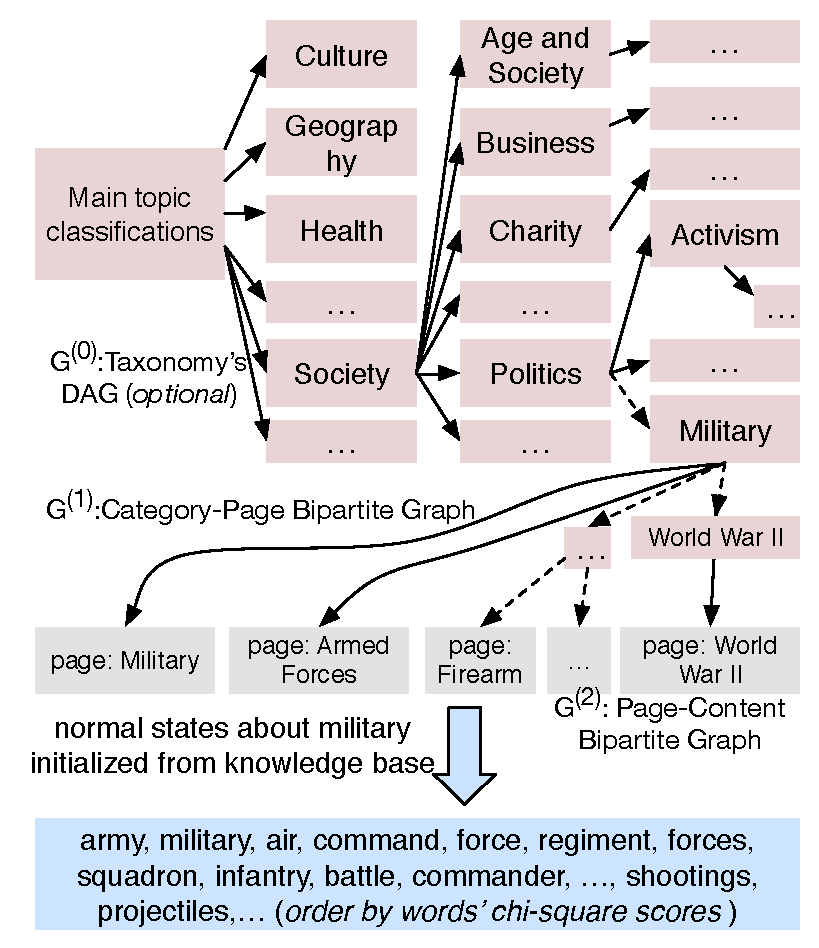
\includegraphics[width=.85\columnwidth]{img/initializationExample.pdf}  
    \caption{Illustration on how to train normal states from wikipedia,( an approximation to the full history information).}
    \label{fig:modelDesc}
\end{figure}


\subsection{Normal States' Maintenance}
KB-Prior-LDA
\begin{figure}[t]
    \centering
    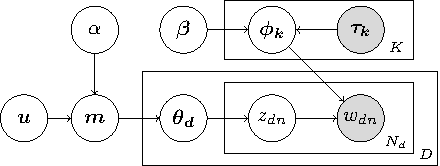
\includegraphics[width=0.75\columnwidth]{model/lda_tikz.pdf}
    \caption{Probabilistic model for training normal states by using history information.}
    %The convolution neural network for extracting character-level representations of words. Dashed arrows indicate a dropout layer applied before character embeddings are input to CNN.}
    \label{fig:cnn}
\end{figure}

\ \ Our theme modeling, want to learn the first \(k\) topics with Wikipedia Article \(k\) topics as close as possible, and we will be Wikipedia article \(k\) before 1000 words) was added to the theme of the word frequency word in the subject a priori distribution on the.
Learning to be the first \(k\) Subject polynomial distribution of the word, referred to as \(\phi_k \), Wikipedia article \(k \) distribution of topics for \(\tau_k \), then this formalized process is expressed as: \(\ \phi_k \sim Dir(\beta + \tau_k) \).
Formal presentation of the explanation is: With prior knowledge \(\tau_k \) after the theme \(\phi_k \) is no longer simply rely on symmetric priori \(\beta \), different words right is not the same weight , such as a discussion of "fashion" theme in Wikipedia, it will refer to "dress", "grand", "blue", "gold" and other words, with the asymmetric priori \(\beta + \tau_k \) after in microblogging "fashion" theme "dress" the proportion will be increased in this way so that microblogging corpus theme tends to Wikipedia topic.
\(\tau_k \) in the first \(v \) words such as formula (\ref{eq: wikiPrior}).
Where \(S_k \) as a set of candidate words: high-quality information to use Wikipedia, we extract the theme \(phi_k \ \) in the higher-word word frequency candidate set \(S_k \).
We can control set \(S_k \) in size, the size of the control is usually set for 1000.
The number of frequency \(n_{kv} \) for the word \(v \) (\ k) appears in the Wikipedia article themes of: (\ref{wikiPrior eq}).
If the word \(v \) does not appear in the candidate set \(S_k \), and then set a priori knowledge \(\tau_{kv} = 0 \), otherwise, the word frequency is proportional to \(n_{kv} \) with the prior knowledge of weight \(W\).
In the latter experiment, we will be on a priori knowledge of weights \(W \) will be discussed. 

\begin{table}[!htbp]
\begin{tabular}{l}
1. Draw corpus prior distribution \(\bm{m} \sim Dir(\alpha \bm{u})\), where \(\bm{u}\)\\
 \ \ \ \ is the uniform distribution. \\
2. For each topic \(k \in \{1,\cdots,K\}\),\\
\ \ \ \ (a) word distribution on the topic \(\bm{\phi_k} \sim Dir(\bm{\beta}+ \bm{\tau_k})\). \\
    
3. For each document index \(d \in \{1,...,D\}\), \\
\ \ \ \ (a) topic distribution on the document \(\theta_d \sim Dir(\bm{m})\), \\
\ \ \ \ (b) for each word index \(n \in \{1,\cdots,N_d\}\),\\
\ \ \ \ \ \ \ \ i. word's topic assignment \(z_{dn} \sim Multinomial(\theta_d)\), \\
\ \ \ \ \ \ \ \ ii. word \(w_{dn} \sim Multinomial(\phi_{z_{dn}})\). \\
\end{tabular}
\end{table}

\begin{scriptsize}
\begin{equation}
\label{eq:wikiPrior}
\begin{aligned}
\tau_{kv}=
\left\{ \begin{aligned}
\lambda \frac{f_{kv}}{\sum_{v\in S_{kv}}f_{kv}} &,v\in S_{k}\ and  \ k \leq K_{\bm{KB}} \\
0&,v \notin S_{k} \ or \ k > K_{\bm{KB}} \\
\end{aligned}\right.
\end{aligned}
\end{equation}
\end{scriptsize}

\begin{scriptsize}
\begin{equation}
\label{eq:initProbability}
\begin{aligned}
\hat{q}_{k|v}=
\left\{ \begin{aligned}
\frac{\tau_{kv}}{\sum_{k=1}^{K}\tau_{kv}} &,\sum_{k}\tau_{kv}>0 \\
0&, \sum_{k}\tau_{kv}=0 \ and \ k \leq K_{\bm{KB}} \\
1/(K-K_{\bm{KB}})&,\sum_{k}\tau_{kv}=0 \ and \ k > K_{\bm{KB}}
\end{aligned}\right.
\end{aligned}
\end{equation}
\end{scriptsize}

\begin{scriptsize}
\begin{equation}
\label{eq:KBPriorLDAgibbs}
\begin{aligned}
&p(z_{dn}=k|w_{dn}=v,z_{\neg{dn}},w_{\neg{dn}},\alpha\bm{m},\beta,\tau)\\
&\ \ \propto (n^{(d)}_{dk}+\alpha m_k)\frac{n^{(w)}_{kv}+\tau_{kv}+\beta}{n^{(w)}_{k,.}+\tau_{k,.}+V\beta}
\end{aligned}
\end{equation}
\end{scriptsize}

\begin{algorithm}
\caption{NS-Prior-LDA Learning Algorithm}
\label{alg:gibbsSamplingKBPriorLDA}
\KwIn{Documents \(\mathcal{D}\) (a.k.a., \(\bm{w_{1:D}}\)), and normal states \(\bm{f}_{1:K_{\bm{KB}}}\)}
\KwOut{The sufficient statistics \(\bm{n^{(d)}}\), \(\bm{n^{(w)}}\)}
\tcc{Initialization of NS-Prior-LDA}
\For{\(d=1:D\)}{
    \For{\(n=1:N_d\)}{
        \(v=w_{dn}\), sample \(z_{dn}=k\) as Eq(\ref{eq:wikiPrior})(\ref{eq:initProbability}).\\
        Update the sufficient statistics \(n^{(d)}_{d,k}\), \(n^{(w)}_{k,v}\).\\
            }
        }
\For{\(i= 1:I\)}{
    \tcc{E-Step of NS-Prior-LDA}
    \For{\(i=1:I_E\)}{
        \For{\(d=1:D\)}{
            \For{\(n=1:N_d\)}{
                Set \(v=w_{dn}\), and reset the sufficient statistics \(n^{(d)}_{d,z_{dn}}\), \(n^{(w)}_{z_{dn},v}\).\\
                Resample \(z_{dn}=k\) as Eq(\ref{eq:wikiPrior})(\ref{eq:KBPriorLDAgibbs}).\\
                Update the sufficient statistics \(n^{(d)}_{d,k}\), \(n^{(w)}_{k,v}\).\\
            }
        }
    }
    \tcc{M-Step of NS-Prior-LDA}
    Optimize \(\alpha \bm{m}\) by the fixed-point iteration\cite{wallach2008structured}. 
}
\Return{\(\bm{n^{(w)}}\)}
\end{algorithm}

\cite{wallach2008structured}\footnote{\url{https://github.com/mimno/Mallet/blob/master/src/cc/mallet/types/Dirichlet.java}}

\subsection{Detecting Events from Normal States}
The state of attention of social issue k at time t in cyberspace is binary, namely at the peak or not at the peak. We denote it by hidden binary variable sk,t, which is 1 or 0. We do the inference for the hidden variable sk,t according to Poisson distribution according to Reference10,11. If the state of attention of social issue k at time t is "not at peak", then the probability density function is 
\(p([Ax_(k,t) ]|s_(k,t)=0)=e^(-μ_0 )  μ_0^([Ax_(k,t)])/([Ax_(k,t)]!)\) otherwise the probability density function is \(p([Ax_(k,t) ]|s_(k,t)=1)=e^(-μ_1 )  μ_1^([Ax_(k,t)])/([Ax_(k,t)])\)
In the above functions the symbol \(x_{k,t}\) denotes the attention of social issue k at time t , the symbol A denotes the constant, \(μ_0\) and \(μ_1\) represent the average of \([Ax_(k,t)]\) at peak and not at peak respectively. The state sk,t is inferred from \(ratio=p([Ax_(k,t) ]|s_(k,t)=0)/p([Ax_(k,t) ]|s_(k,t)=1) \).
In calculation, we use the log ratio to determine whether the attention is at peak as in equation (1). logratio>0 indicates that the attention of social issue k at time t is not at peak, otherwise at peak. As the attention xk,t is often between 0.01% and 5% in our experiment, we set the constant A in log ratio equation to be〖10〗^4。
	\(logratio=-(μ_0-μ_1 )+[Ax_(k,t)](log⁡μ_0 -log⁡μ_1)\)
After the data preprocessing, we get the air pollution state sequence\((a_t)_(t=1,…T)\) and the attention state sequence of each social issue \((s_(k,t))_(t=1,…,T;k=1…n)\), where T denotes the number of time windows.

\begin{algorithm}
\caption{Spectral Clustering Based Event Phrase Extraction}
\label{alg:eventKeywordsSearchMethod}
\KwIn{\(\mathcal{B}_{k,t},\mathcal{G}_{k,t},\rho\)}
\KwOut{\(\mathcal{C}_{k,t}\)}
\(n_{k,t}\)=number of connected component in \(\mathcal{G}_{k,t}\)\\
\For{\(n \in \{ n_{k,t}, \cdots, |\mathcal{G}_{k,t}|\}\) }{
    \(\mathcal{C}_{k,t}=SpectralClustering(\mathcal{G}_{k,t},n)\)\\
    \If{\(min_{i\in \{1,\cdots,n\}} Density(\mathcal{C}_{k,t,i},\mathcal{G}_{k,t})>\rho\)}{
        return \(\mathcal{C}_{k,t}\)
    }
}
\end{algorithm}


\begin{figure}
\centering
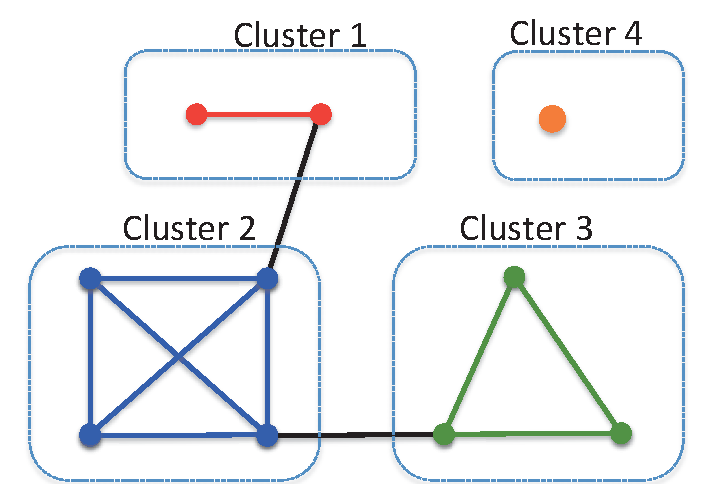
\includegraphics[height=3cm]{img/wordClusterGraph.eps}
%todo
\caption{Hot words between the heat pattern forming word time window edge weight calculated by the PMI obtained between words, to obtain spectral clustering clustering clustering}
\label{fig: windowsBurstyWordGraph}
\end{figure}

\textbf{event} phrase Mining
% Refer to bursty.py
\ \ Microblogging mining events can be represented by a variety of ways, a single word, phrase, or topic.
Here we use the form of phrase, said event.
In this paper, the phrase indicates that the event is due to the fact that: the same period of time when there are multiple areas of internal hot words appear, a collection of hot words \(\mathcal{B}_{k, t} \) between the hot words great probability is interrelated. For example, observed "mac", "os", "lion" three words are in a state of emergency.
In fact, the state of emergency three words is to publish a new system "mac os lion" event caused by Apple, in order to find the association between words and events, we use spectral clustering based search methods.

As shown in Figure \ref{fig: windowsBurstyWordGraph} below, we will one area, a hot word of the time window and hot words between to diagram.
Hot words set \(\ mathcal{B}_{k, t} \) formed in FIG using \textbf{hot word graph} \(\mathcal {G}_{k, t} = (\mathcal{B}_{k, t}, \mathcal{E}_{k, t}) \) indicates,
\(\mathcal{E}_{k, t} = \{(a, b) | a \in \mathcal{B}_{k, t}, b \in \mathcal {B} _ {k, t }, PMI (\mathcal{D}_{k, t}, a, b)> 0 \} \), where \(PMI (\mathcal{D}_{k, t}, a, b) \) the field \(k \) time window \(t \) related microblog \(\ mathcal {D} _ {k, t} \) on the word \(a \) and the word \(b \) point metric information between each other.
% Refer to bursty.py getSimGraph () function

Given a field \(k \) and the time window \(t \), in which the number of events can not be determined in advance.
The two most extreme situations are: events coarse granularity, said the event is equal to the number of Figure \(\ mathcal {G} _ {k, t} \) in the number of connected components; events finer granularity display, event number equal to \(\ mathcal {G} _ {k, t} \) the number of points.
To do this, we use the Density to the degree of density of quantum graphs \(2 \#Edge / (\# Node \ cdot (\# Node-1)) \), the more the greater if the edge density in the range of Density in \((0,1] \).
Density can be a good indicator to determine the size indicates the event: too many unrelated phrases to put together an event can not be represented, too fine particle size, such as a single word can represent only part of the event; only in close co-occurrence of the phrase to a reasonable It indicates that the event granularity.
To this end, we have designed events phrase search algorithm \ ref {alg: eventKeywordsSearchMethod}: We try to find a reasonable number of spectral clustering Clustering \(n \), let \(n \) from a smaller value ( event corresponds to coarser granularity representation) to start the search, then the most likely cluster cluster size is too large, its performance is the clustering results in one or more small Density indicators; continue to increase the number of clusters \(n \), the event represents reduced size, reduced the size of clusters of clusters, thus making the Density index increases; when all cluster clustering Density indicators are larger than the threshold \(\tau \), the search terminates, returning clustering results \(\mathcal{C}_{k, t}\).
As the above process algorithm \ref{alg: eventKeywordsSearchMethod} description line 2 to line 5, we use in practice \(\tau = 0.6 \).
We call \(\mathcal{C}_{k, t} \) results in each cluster to cluster \textbf{event} phrase.

\textbf{detected events related to micro-blog}
\ \
By algorithm \ref{alg:eventKeywordsSearchMethod} find art \(k \) time window \ \(t \) within the \(| \mathcal{C}_{k, t} | \) events phrase later, you can also further find each event and the corresponding event phrase microblogging.
We looked at the first \(i \) events phrase \(\mathcal{C}_{k, t, i} \),
The phrase based on the number of elements distinguish the event, there are three situations: (1) the phrase event more than two hot words, he said while the event is not a phrase between any two words We have a very strong relationship between the co-occurrence, so just pay attention to the co-occurrence relationship stronger side; (2) event phrase has two hot words; (3) the event is only a hot word in the phrase.
Weibo text length is shorter, not all of the microblogging event will include the phrase \(\mathcal{C}_{k, t, i} \) in all the words.
Such as those on "Apple released the new system mac os lion" event, the event phrase "mac", "os", "lion" does not need to appear in all of the micro-Bo, just check the co-occurrence of a strong relationship between the two words appear together whether in an article in the field \(k \) time window \(t \) micro-Bo: If there is, then added to the events related to the collection \(\ mathcal {D} _ {k, t, i} \) in.
For the case of a third cluster cluster contains only a hot word, we only need to identify areas \(k \) contains the hot word of all micro-blog, and add the event to the relevant set \(\ mathcal{D }_{k, t, i} \) in.
Ultimately, we can get the field \(k \) next time window \(t \) in the event the phrase relating to events microblogging \(\{(\mathcal{C}_{k, t, i}, \mathcal{D}_{k, t, i}) \}_{i=1}^{| \mathcal{C}_{k, t} |} \).

\section{Experiments}
\begin{figure}
        \centering
        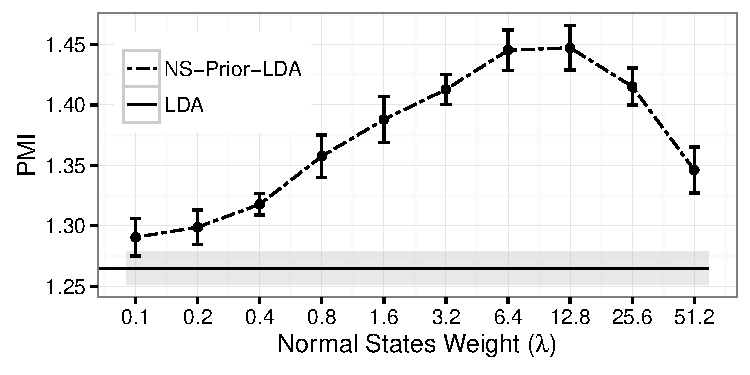
\includegraphics[height=4.0cm]{img/pmi.pdf}
        \caption{The quality of all twitter topics learned by NS-Prior-LDA increases with normal states weight (\(\lambda\)) before \(\lambda=12.8\). The optimized PMI is gained with moderate normal states weight when considering topics \(k\leq K_{\bm{KB}}\) and topics \(k > K_{\bm{KB}}\) together.}
\end{figure}

\begin{table}
\centering
\caption{The PMI of twitter topics learned by NS-Prior-LDA, its variant, and other baselines}
    \begin{tabular}{|l|l|c|}
    \hline
    Model & Prior Knowledge & PMI \\ \hline
    LDA & None  & 1.265 \(\pm\) 0.013     \\ \hline
    BBTM\cite{Yan:2015wm} & None    & 1.467 \(\pm\) 0.017     \\ \hline
    NS-Prior-LDA\(^{(-)}\)   &   \begin{tabular}[c]{@{}l@{}}\footnotesize{Words in categories simply}\\ \footnotesize{extracted from Wikipedia}\end{tabular} & 1.439 \(\pm\) 0.010     \\ \hline
    NS-Prior-LDA         & \begin{tabular}[c]{@{}l@{}}\footnotesize{Normal states initialized} \\\footnotesize{from wikipedia}\end{tabular} & 1.523 \(\pm\) 0.017     \\ \hline
    \end{tabular}
\label{tbl:NS-Prior-LDA}
\end{table}

\begin{table*}[ht]
\centering
\caption{My caption}
\label{my-label}
\scalebox{0.88}{
\begin{tabular}{|cc|cc|cc|cc|cc|cc|}
\hline
\multicolumn{2}{|c|}{\textit{Aviation}} & \multicolumn{2}{c|}{\textit{Health}} & \multicolumn{2}{c|}{\textit{Middle East}} & \multicolumn{2}{c|}{\textit{Military}} & \multicolumn{2}{c|}{\textit{Mobile Phones}} & \multicolumn{2}{c|}{\textit{Video Games}} \\
\begin{tabular}[c]{@{}c@{}}Normal\\ States\end{tabular} & \begin{tabular}[c]{@{}c@{}}Topical\\ Words\end{tabular} & \begin{tabular}[c]{@{}c@{}}Normal\\ States\end{tabular} & \begin{tabular}[c]{@{}c@{}}Topical\\ Words\end{tabular} & \begin{tabular}[c]{@{}c@{}}Normal\\ States\end{tabular} & \begin{tabular}[c]{@{}c@{}}Topical\\ Words\end{tabular} & \begin{tabular}[c]{@{}c@{}}Normal\\ States\end{tabular} & \begin{tabular}[c]{@{}c@{}}Topical\\ Words\end{tabular} & \begin{tabular}[c]{@{}c@{}}Normal\\ States\end{tabular} & \begin{tabular}[c]{@{}c@{}}Topical\\ Words\end{tabular} & \begin{tabular}[c]{@{}c@{}}Normal\\ States\end{tabular} & \begin{tabular}[c]{@{}c@{}}Topical\\ Words\end{tabular} \\ 
\hline
aircraft & air\scriptsize(3253) & health & weight\scriptsize(16344) & al & \textcolor{red}{\textit{\#syria}}\scriptsize(4212) & army & killed\scriptsize(4055)  & android & iphone\scriptsize (13674) & game & games\scriptsize(8812) \\ 
air & plane & patients & loss & israel & \textcolor{red}{\textit{\#bahrain}} & military & news & mobile & apple & player & liked \\ 
airport & flight & medical & diet & iran & people & air & \textcolor{red}{\textit{\#libya}}\scriptsize(3503) & nokia & android & playstation & free \\ 
flight & time & disease & health & arab & israel & command & libya & ios & app & gameplay & xbox \\
airline & airlines & treatment & cancer & israeli & police & force & rebels & phone & ipad & nintendo & 360 \\
airlines & news & hospital & lose & egypt & \textcolor{red}{\textit{\#libya}}\scriptsize(2557) & regiment & people & samsung & samsung & games & playing \\
aviation & boat & patient & fat & egyptian & \#egypt & forces & police & game & mobile & players & played \\
flying & airport & clinical & tips & ibn & news & squadron & war & app & blackberry & xbox &iphone\scriptsize(2820)\\
pilot & force & symptoms & treatment & jerusalem & \#israel & infantry & libyan & iphone & tablet & mode & time\\
squadron & fly & cancer & body & syria & world & battle & attack & htc & apps & arcade & \textcolor{red}{\textit{ps3}}\\
flights & hurricane & cells & healthy & iraq & syria & commander & u.s. & smartphone & free & wii & trailer\\
pilots & navy & blood & study & palestinian & protest & ship & gaddafi & phones & \#android & multiplayer & online\\
raf & flying & therapy & pain & syrian & israeli & corps & army & blackberry & htc & sega & hours\\
airways & aircraft & drug & exercise & iranian & egypt & navy & forces & apps & google & console & ipad\\
fighter & \textcolor{red}{\textit{irene}} & medicine & \#health & ottoman & al & brigade & pakistan & ipad & galaxy & enemies & app\\
boeing & crew & brain & natural & islamic & syrian & battalion & afghanistan & gsm & ios & characters & player\\
runway & sky & care & disease & iraqi & protesters & lieutenant & military & lte & store & playable & wii\\
force & crash & syndrome & acne & abu & arab & aircraft & attacks & symbian & windows & character & ops\\
crashed & jet & infection & hair & jewish & rights & officer & troops & devices & mac & video & download\\
flew & pilot & disorder & surgery & persian & libya & naval & dead & smartphones & phones & graphics & nintendo\\
\hline
\end{tabular}
}
\end{table*}

\begin{table*}[ht]
\centering
\caption{My caption}
\label{my-label}
\subtable[Twitter Dataset Statistics]{
\begin{tabular}{|l|r|}
\hline
Time range & \begin{tabular}[c]{@{}l@{}}2011/06/30\\ -2011/09/15\end{tabular} \\ \hline
Tweet Number & 36,627,434 \\ \hline
\begin{tabular}[c]{@{}l@{}}Event Number \\ in Benchmark1\end{tabular} & 27 \\ \hline
\begin{tabular}[c]{@{}l@{}}Event Number \\ in Benchmark2\end{tabular} & 523 \\ \hline
\end{tabular}
}\quad \quad
\subtable[Event Detection Results]{
    \begin{tabular}{|l|l|l|l|l|}
    \hline
    Method & \begin{tabular}[c]{@{}l@{}}Recall@ \\ Benchmark1\end{tabular} & \begin{tabular}[c]{@{}l@{}}Precision@ \\ Benchmark2\end{tabular} & \begin{tabular}[c]{@{}l@{}}Recall@ \\ Benchmark2\end{tabular} & \begin{tabular}[c]{@{}l@{}}DERate(Duplicate \\ Event Rate)\end{tabular} \\ \hline
    UMass System & 0.882 & 0.138 & 0.941 & 0.071 \\ \hline
    LSH & 0.824 & 0.095 & 0.803 & 0.302 \\ \hline
    TimeUserLDA & 0.353 & 0.536 & 0.071 & 0.054 \\ \hline
    Twevent & 0.824 & 0.697 & 0.641 & 0.113 \\ \hline
    EDCoW & 0.412 & 0.756 & 0.119 & 0.290 \\ \hline
    BBTM & 0.647 & 0.809 & 0.170 & 0.045 \\ \hline
    \textsc{NSDetector} & 1.000 & 0.894 & 0.950 & 0.042 \\ \hline
    \end{tabular}
}
\end{table*}

\begin{table*}[ht]
\centering
\caption{Events about \textit{vehicles} detected by systems between 2011-07-20 and 2011-07-30}
\label{my-label}
\begin{tabular}{|l|L{3cm}|l|c|}
\hline
\multicolumn{1}{|c|}{Date} & \multicolumn{1}{c|}{Event key words} & \multicolumn{1}{c|}{Representative event tweet} & \multicolumn{1}{c|}{\begin{tabular}[c]{@{}c@{}}Number of \\ event tweet\end{tabular}} \\ \hline
7/20/11 & \begin{tabular}[c]{@{}l@{}}American, airlines, \\ order, planes\end{tabular} & \begin{tabular}[c]{@{}l@{}}NDTV: American Airlines orders 460 new planes from \\ Boeing, Airbus http://bit.ly/p1ZgYG\end{tabular} & 31 \\ \hline
7/26/11 & \begin{tabular}[c]{@{}l@{}}Morocco, military, \\ plane, crash\end{tabular} & \begin{tabular}[c]{@{}l@{}}BBC News - Morocco military plane crash kills 78 \\ http://t.co/uwnLv8L\end{tabular} & 36 \\ \hline
7/27/11 & air, Canada & \begin{tabular}[c]{@{}l@{}}Smoke in galley forces Air Canada flight back to airport. \\ Plane landed safely in Sydney, Australia after dumping fuel\end{tabular} & 48 \\ \hline
7/30/11 & \begin{tabular}[c]{@{}l@{}}Caribbean, airlines, \\ crashes, Guyana\end{tabular} & \begin{tabular}[c]{@{}l@{}}Caribbean Airlines Jet Crash-Lands In Guyana All 163 \\ Passengers, Crew Survive http://t.co/qPVD3WJ\end{tabular} & 57 \\ \hline
\end{tabular}
\end{table*}

\begin{table*}[ht]
\centering
\caption{Events about \textit{military} detected by systems between 2011-07-20 and 2011-07-30}
\label{my-label}
\begin{tabular}{|l|L{3cm}|l|l|}
\hline
Date & Event key words & Representative event tweet & \begin{tabular}[c]{@{}l@{}}Number of \\ event tweet\end{tabular} \\ \hline
7/20/11 & \begin{tabular}[c]{@{}l@{}}Serbia, crimes, \\ fugitive, arrests\end{tabular} & Serbia: Serbia arrests last war crimes fugitive-TV- Reuters & 27 \\ \hline
7/20/11 & Somalia, famine & \begin{tabular}[c]{@{}l@{}}UN declares famine in Somalia. What can we do to save \\ 3.7million lives? http://bit.ly/r1Rq7R\end{tabular} & 89 \\ \hline
7/21/11 & \begin{tabular}[c]{@{}l@{}}U.S., military, \\accept, gay, \\lesbian, openly\end{tabular} & \begin{tabular}[c]{@{}l@{}}RT @cnnbrk: Pentagon is set to certify that the U.S. military \\ is prepared to accept openly gay and lesbian service members \\ \#dadt\end{tabular} & 20 \\ \hline
7/22/11 & \begin{tabular}[c]{@{}l@{}}Norway, Oslo,\\ attacks, bombing\end{tabular} & \begin{tabular}[c]{@{}l@{}}Terror Attacks Devastate Norway: A bomb ripped through \\ government offices in Oslo and a gunman...˙http://dlvr.it/cLbk8\end{tabular} & 557 \\ \hline
7/23/11 & Gunman, rink & \begin{tabular}[c]{@{}l@{}}Gunman Kills Self, 5 Others at Texas Roller Rink \\ http://dlvr.it/cLcTH\end{tabular} & 43 \\ \hline
7/26/11 & \begin{tabular}[c]{@{}l@{}}Kandahar, mayor, \\ suicide, attack\end{tabular} & \begin{tabular}[c]{@{}l@{}}TELEGRAPH{]}: Kandahar mayor killed by Afghan suicide \\ bomber: The mayor of Kandahar, the biggest city in south \_\end{tabular} & 25 \\ \hline
7/28/11 & Ft., Hood, attack & Possible Ft. Hood Attack Thwarted http://t.co/BSJ33hk & 20 \\ \hline
7/28/11 & \begin{tabular}[c]{@{}l@{}}Libyan, rebel, \\ gunned\end{tabular} & \begin{tabular}[c]{@{}l@{}}Libyan rebel chief gunned down in Benghazi \\ http://sns.mx/prfvy1\end{tabular} & 44 \\ \hline
\end{tabular}
\end{table*}

\begin{figure*}
    \label{fig:algorithm}
    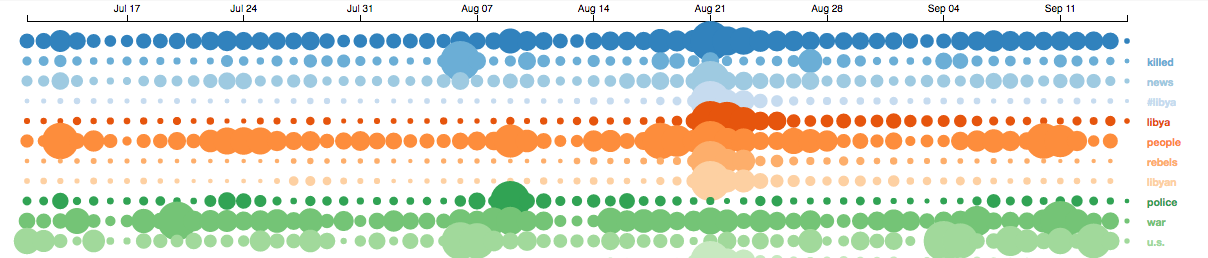
\includegraphics[width=1.0\textwidth]{img/screenShot.png}
    \caption{An illustration of the time series of Military related states on Twitter dataset from 2011-06-30 to 2011-09-15.}
\end{figure*}

\subsection{Data set and experiment settings}
\textbf{Data set.} We conduct the empirical analysis on a twitter dataset which is constructed by \cite{petrovic2012using} and widely used by previous event detection researches \cite{petrovic2013can} \cite{Wurzer:2015wq}. 
Due to the developer policy of Twitter\footnote{https://dev.twitter.com/overview/terms/policy}, \cite{petrovic2012using} only redistributes tweets' IDs\footnote{http://demeter.inf.ed.ac.uk/cross/docs/fsd\_corpus.tar.gz}.
We collected the tweets' contents according to the IDs with the help of Twitter API. 

%TODO
The benchmark \textit{Edinburgh twitter corpus} contains 27 manually labeled events\cite{petrovic2013can}\footnote{\url{http://demeter.inf.ed.ac.uk/cross/docs/Newswire_Events.tar.gz}} and 90 million tweets. Though we cannot get the whole dataset due to the limit of Twitter API, after neccessary pre-processing, our rebuilt dataset still contains 36,627,434 tweets, which spans identically from 2011/06/30 to 2011/09/15, and also covers 27 labeled events.
More details of the original dataset are described in \cite{petrovic2010edinburgh}.

20-newsgroup\footnote{http://qwone.com/~jason/20Newsgroups/}

\textbf{Benchmark1} The first set of the ground truth about events in the corpus are provided by \cite{petrovic2013can}, which is mentioned above. 
And 27 events ...

\textbf{Benchmark2} here.

\textbf{Normal States Initialization} here.

\textbf{Baseline}

UMass System

LSH

TimeUserLDA

Twevent

EDCoW

BBTM

\textbf{Model Setting}

\subsection{Validity of Normal States}
\textbf{Topic Coherence} \cite{roder2015exploring}
\subsection{Topical Words Learned by NS-Prior-LDA}
\textbf{PMI}
\subsection{Evaluation of Detected Events}
\textbf{Precision} Precision@Benchmark1, Precision@Benchmark2

\textbf{Recall}

\textbf{Accuracy}

\textbf{DERate(Duplicate Event Rate)}
\subsection{Case Study}


Here we present the effectiveness of our proposed algorithm UMIETM and the efficiency of its online performance.
We evaluate the efficiency by perplexity, precision for event detection. 
We check the time cost and complete likelihood for efficiency.

To improve the quality of analyzing on tweets, we do necessary pre-processing: (1) splitting dataset by week, (2) segmenting Chinese words, (3) removing stop words and low frequency words whose document frequency in its time window is less than 3.

We compare our model UMIETM with twitterLDA, timeUserLDA, Author-LDA, and our model's variant IETM.
Author-LDA combines the tweets posted by same author into a single document, then run standard LDA on the assembled tweets.
TwitterLDA is designed for topic modeling on twitter.
We compare with Author-LDA and TwitterLDA for confirming the significance of distinguishing user interests from events in microblog.
TimeUserLDA is designed for retrospective event detection in microblog, and considers to distinguish events from user interests.
We compare with timeUserLDA to show the impact of user profile.
The variant IETM (\textit{Interest and Event Topic Model}) models user's interests and events without the help of user profiles.

We set the asymmetric \(\alpha\) and symmetric \(\beta=0.01\) for UMIETM, where \(\alpha\) will be optimized by Gibbs EM algorithm\cite{wallach2008structured}.
\(\alpha=0.1\), \(\beta=0.01\) are set for all remaining models. 
After cross validation we find that UMIETM and IETM perform best on \(K=90\) and \(E=30\), \(\kappa=0.01\).
To compare equally, we set the same topic number for Author-LDA, twitterLDA, timeUserLDA (which means when we run models offline on 1 time window, we shall set 120 topics for all, and 150 topics on 2 time windows and so on).

To verify the role of user profiles played, we set UMIETM(-) as the degradation of UMIETM, which take symmetric prior \(\alpha\).

In this subsection, we illustrate the performance of UMIETM in which user profile is considered.

\textbf{Quantitative Measure.}
We initialize UMIETM and IETM by batch learning on data from first week to third week, then run them in online learning way from fourth week to ninth week.
On each week we calculate their perplexities\cite{wallach2009evaluation}, where \(perplexity(D_{test})=\exp{\{-\frac{\sum_{u=1}^{U}\sum_{d=1}^{D_u}\log{p(w_{ud})}}{\sum_{u=1}^{U}\sum_{d=1}^{D_u}N_{ud}}\}}\) and \(p(w_{ud})=(1-\pi_u)\sum_{k=1}^{K}\theta_{uk}\prod_{n=1}^{N_{ud}}(\phi_{s,w_{udn}}(1-\rho)+\phi_{k,w_{udn}}\rho)+\pi_u \sum_{k=1}^{K}\eta_{t,k}\prod_{n=1}^{N_{ud}}(\phi_{s,w_{udn}}(1-\rho)+\phi_{k,w_{udn}}\rho)\).
The others are trained from first week to third week, and the held out perplexities are calculated on data from fourth week to ninth week.
TimeUserLDA and IETM's perplexities are smaller than User-LDA, twitterLDA as they both consider distinguishing user interests from events.

In Table \ref{tab:heldoutPerplexity} the perplexity of UMIETM is 3107.8, and much smaller than others. It demonstrates that user profile is significant for tweet stream's modeling.

In Table \ref{tab:metrics}, we evaluate the events detected by models. We asked the annotators to label the event with score 1, and non-event related topic as 0. 
The precision and recall is illustrated, where UMIETM(-) performs slightly better than IETM. 
And UMIETM outperforms UMIETM(-) in detecting high quality event. 
A reasonable analysis is that UMIETM uses the profile information sufficiently by asymmetric priors. 
In this way, we also prove that the well exploiting of user profile information is important to model user interests and events on tweets. 
%\subsubsection{Precision of Event Detection}

\textbf{Case Study} 
Some events detected by our UMIETM model are shown in Table \ref{fig:event}.
Comparing with UMIETM, timeUserLDA fails to discover the \textit{shoddy construction} event in the second week, while IETM reports this event as \textit{bi, women, elegant, adoption, engineering, reed}. Obviously IETM fails to distinguish this event from user interests.
UMIETM filters users' interests like \textit{bi, women, elegant, adoption} using their profile {\#baby, \#women}, and detect the event.
\subsection{Efficiency}
We implement our methods on mallet\footnote{http://mallet.cs.umass.edu/dist/mallet-2.0.7.tar.gz}, and run them on Linux server with 8 cores(2.00GHz) and 64GB memory.
In this subsection, we verify the convergence and online performance of our online learning algorithm. 

\textbf{Convergence.}
The convergence of algorithm is vital in real time streaming environment. 
UMIETM needs several Gibbs sweeps to find out the optimal parameters of model.
But the size of data is usually large even spitted into time windows.
The time complexity of UMIETM is \(O(I_1K|P|+I_2K|W|+I_2E|W|)\) given in section \ref{subsec:online}.
It suggests that the more iterations Gibbs sampling have to do, the less efficiently our model performs. 
Fortunately UMIETM is very economic to its stable state and does not need so much iterations.
As suggested by \cite{wallach2009rethinking} and \cite{jian2014factorOfTopicModel}, we choose LDA with asymmetric priors as baseline, which is much more comparable than standard LDA on microblog dataset.
We run UMIETM on the first three time windows. 
Correspondingly we only use the tweets in these time windows for LDA with asymmetric priors.
Burn-in period is set to 20 and optimize interval also 20, which means the priors are optimized every 20 iterations as the red curve in Fig \ref{fig:completeLoglikelihood}.

One of the criteria for stopping Gibbs sampling is that the complete log likelihood is stabilized.
We stop UMIETM after 50 iterations since the complete log likelihood only increases 0.02\% in last iteration.
It will take LDA(asymmetric priors) 300 minutes to run 1000 iterations, and 20 minutes per 10 iterations for UMIETM.
There is a trade-off between the effectiveness by more iterations and efficiency by less,  we set the iteration number as 10 in online setting.
After 10 iterations the UMIETM's complete log likelihood will increase no more than 0.2\%.

\textbf{Online Performance.}
As verified in the above subsection \textit{Convergence}, we run 10 Gibbs sweeps for each time window in online learning phase.
When UMIETM is implemented in online way, it doesn't have to revisit the tweets in previous windows. 
So its time cost in each window is proportional to the data size of current window  as shown in Figure \ref{fig:onlinelearningResult}.
In average, online UMIETM can process five thousand tokens per second.
%Memory cost grows slightly and the increased memory cost only depends on the size of vocabulary.

LSH based event detection on microblogs is used by \cite{petrovic2010streaming},\cite{mccreadiescalable}. 
The former one detects events as the cluster of tweets by LSH, and the latter one extends this method on distributed machines. 
They both only use the cosine similarity without considering semantic meaning of words. 
So LSH based method may split the same event into clusters of similar tweets.
However LSH based method reports 10578 events in 7th time window, and 10901 events in 8th window. 
The other problem of LSH based event detection method is that the bad design may lead unstable performance. 
The tweets are mapped into LSH defined space in a skew way which is illustrated in Fig \ref{fig:onlinelearningResult}.
The other comparison is timeUserLDA which is designed for retrospective event detction. 
The purple line in Fig \ref{fig:onlinelearningResult} goes up straightly as timeUserLDA has to revisit previous tweets to make a decision whether the tweet is event related. 
The perplexity of online UMIETM on the 11 time window in Fig \ref{fig:onlinelearningResult} is \(3036.44\pm397.14\). 
And the average precision of detecting high quality event is 0.22.
Both indicators demonstrate that UMIETM can perform well in online learning way. 
\subsection{Application on Reddit}

\section{Conclusions \& Future Work}
Microbiolog is mixed with user interests and external events.
The quality of event detection in microblog depends on how we distinguish them.
We exploit user profile to discover events by filtering out user interest-related tweets.
We further treat the arriving data as stream and run the detection in online learning style.
The experiments demonstrates that our method is effective and efficient for online event detection in microblogs.


\bibliographystyle{unsrt}
\bibliography{paperbib}  

\end{document}
